\chapter{Propeller Design}
\section{Introduction}
A relatively simple method of predicting the performance of a propeller (as well as fans or windmills) is the use of Blade Element Theory. In this method the propeller is divided into a number of independent sections along the length. At each section a force balance is applied involving 2D section lift and drag with the thrust and torque produced by the section. At the same time a balance of axial and angular momentum is applied. This produces a set of non-linear equations that can be solved by iteration for each blade section. The resulting values of section thrust and torque can be summed to predict the overall performance of the propeller.
The theory does not include secondary effects such as 3-D flow velocities induced on the propeller by the shed tip vortex or radial components of flow induced by angular acceleration due to the rotation of the propeller. In comparison with real propeller results this theory will over-predict thrust and under-predict torque with a resulting increase in theoretical efficiency of 5\% to 10\% over measured performance. Some of the flow assumptions made also breakdown for extreme conditions when the flow on the blade becomes stalled or there is a significant proportion of the propeller blade in windmilling configuration while other parts are still thrust producing.
The theory has been found very useful for comparative studies such as optimising blade pitch setting for a given cruise speed or in determining the optimum blade solidity for a propeller. Given the above limitations it is still the best tool available for getting good first order predictions of thrust, torque and efficiency for propellers under a large range of operating conditions.

\section{Blade Element Subdivision}
A propeller blade can be subdivided as shown into a discrete number of sections.
\begin{figure}[h]
\centering
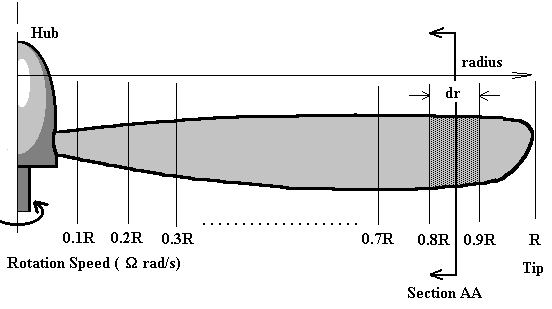
\includegraphics[scale=.7]{blade1.jpeg}
\caption{propeller}
\label{figure}
\end{figure}
For each section the flow can be analysed independently if the assumption is made that for each there are only axial and angular velocity components and that the induced flow input from other sections is negligible. Thus at section AA (radius = r) shown above, the flow on the blade would consist of the following components.
\begin{figure}[h]
	\centering
	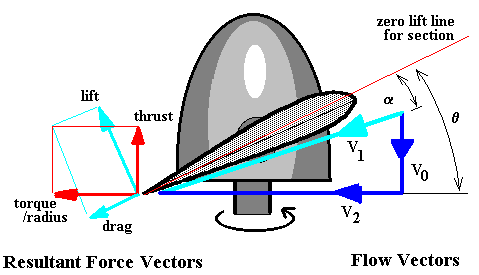
\includegraphics[scale=.8]{blade2}
	\caption{propeller}
	\label{figure}
\end{figure}

$V_{0}$ - axial flow at propeller disk.
$V_{2}$ - Angular flow velocity vector.

$V_{1}$ - section local flow velocity vector, summation of vectors $V_{0}$ and $V_{2}$.

Since the propeller blade will be set at a given geometric pitch angle, the local velocity vector will create a flow angle of attack on the section. Lift and drag of the section can be calculated using standard 2-D aerofoil properties. (Note: change of reference line from chord to zero lift line). The lift and drag components normal to and parallel to the propeller disk can be calculated so that the contribution to thrust and torque of the compete propeller from this single element can be found.

The difference in angle between thrust and lift directions is defined as 
$\phi$ = $\theta$ - $\alpha$

The elemental thrust and torque of this blade element can thus be written as

$\Delta$ T = $\Delta$ L $\cos$ $\phi$ - $\Delta$ D $\sin$ $\phi$

$\dfrac{\Delta Q}{r}$  = $\Delta D \cos \phi + \Delta L \sin \Phi$


Substituting section data (CL and CD for the given   ) leads to the following equations.
per blade
where  is the air density, c is the blade chord so that the lift producing area of the blade element is c.dr.
If the number of propeller blades is (B) then,

\section{Inflow Factors}
A major complexity in applying this theory arises when trying to determine the magnitude of the two flow components $V_{0}$ and $V_{2}$. $V_{0}$ is roughly equal to the aircraft's forward velocity (Vinf) but is increased by the propeller's own induced axial flow into a slipstream. $V_{2}$ is roughly equal to the blade section's angular speed ( r) but is reduced slightly due to the swirling nature of the flow induced by the propeller. To calculate $V_{0}$ and $V_{2}$ accurately both axial and angular momentum balances must be applied to predict the induced flow effects on a given blade element. As shown in the following diagram the induced flow components can be defined as factors increasing or decreasing the major flow components.
\begin{figure}[H]
	\centering
	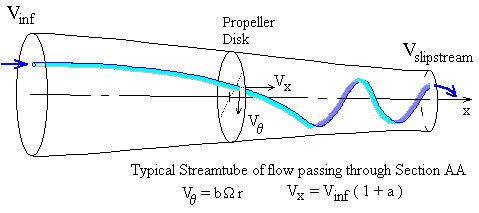
\includegraphics[scale=.7]{blade3}
	\caption{Streamtube of flow}
	\label{figure}
\end{figure}

.









\section{Different Parameters}

\subsection{Coefficient of Thrust}

$C_{To}$=$\dfrac{T}{\rho*n^{2}*D^{4}}$

Where

\begin{itemize}
	
\item  $C_{To}$ = Coefficient of Thrust
\item  T = Thrust
\item  $\rho$ = Density of air
\item  D = Diameter of propeller

\end{itemize} 

\begin{figure}[H]
	\centering
	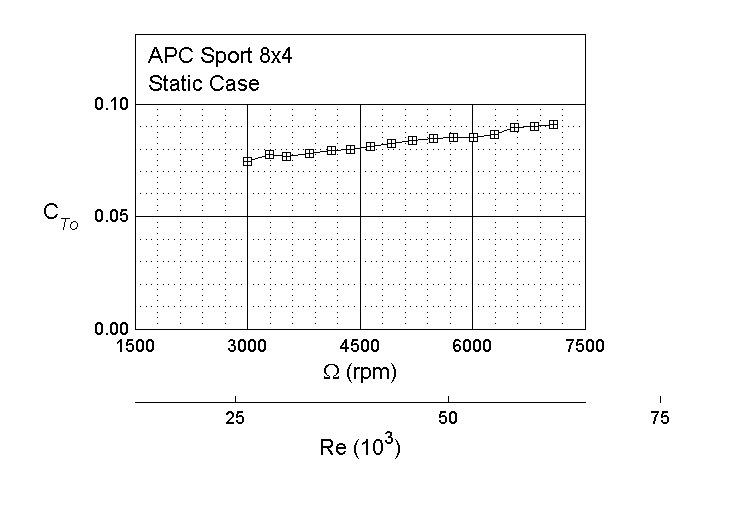
\includegraphics[scale=.5]{graph2}
	
	\caption{$C_{T_{0}}$ Vs  RPM }
	\label{graph}
\end{figure}


\newpage



\subsection{Coefficient of Power}

$C_{Po}$=$\dfrac{P}{\rho*n^{3}*D^{5}}$

Where

\begin{itemize}
	
	\item  $C_{Po}$ = Coefficient of Power
	\item  P = Thrust
	\item  $\rho$ = Density of air
	\item  D = Diameter of propeller
	
	
	
\end{itemize} 





\begin{figure}[H]
	\centering
	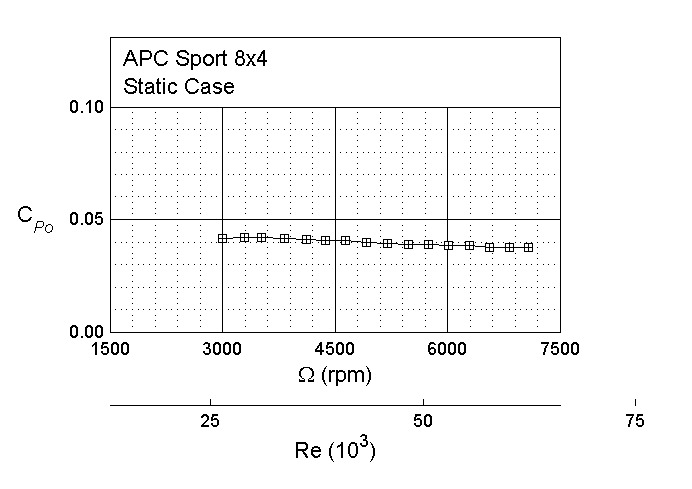
\includegraphics[scale=.5]{graph1}
	\caption{$C_{p_{0}}$ Vs  RPM }
	\label{graph}
	
\end{figure}
\newpage

\subsection{Coefficient of dynamic thrust}

Where   

   J=$\dfrac{V}{nD}$
   
   V = velocity of Drone
   
   
   n= Rotation per Second
   



\begin{figure}[H]
	\centering
	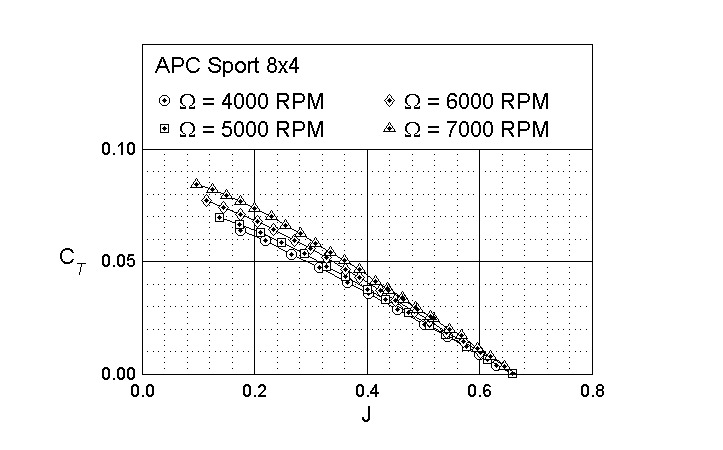
\includegraphics[scale=.5]{graph4}
	\caption{$C_{T}$ Vs J }
	\label{graph}
\end{figure}

\subsection{Efficiency v/s Advance Ratio Graph}
\begin{figure}[H]
	\centering
	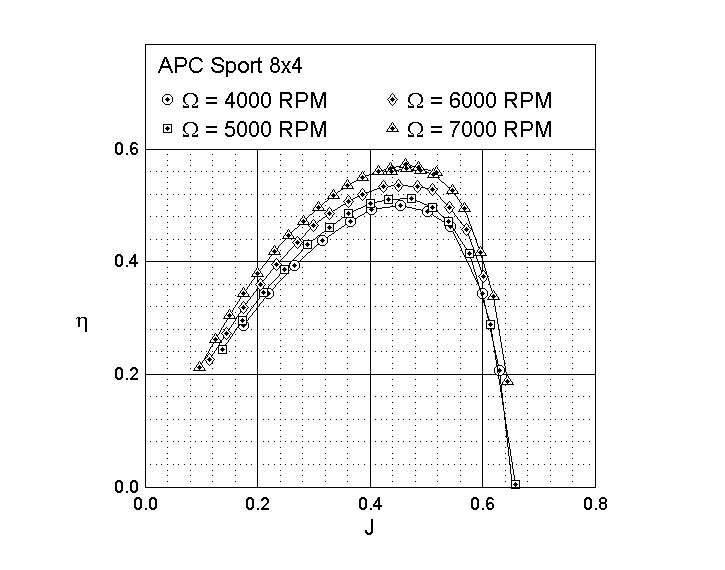
\includegraphics[scale=.7]{graph3}
	\caption{$\eta$  Vs J }
	\label{graph}
\end{figure}

\subsection{Coefficient of dynamic power v/s Advance ration Graph}

\begin{figure}[H]
\centering
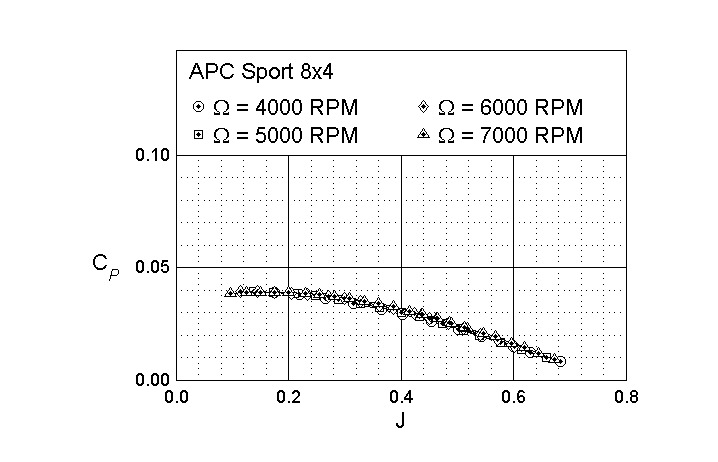
\includegraphics[scale=.7]{graph5}
\caption{$C_{P}$ Vs  J }
\label{graph}
\end{figure}

\newpage

\section{Sample Calculation}

Required Thrust = .284 * 9.81 = 2.786 N


Density of Air = 1.225 Kg/$m^{3}$

RPS (n) = 120

Diameter = 0.2032 m


$C_{T}$ = $\dfrac{2.786}{1.225 * 120^{2} * 0.2032^{4}}$ = 0.0926

$C_{P}$ = 0.039

$C_{Po}$=$\dfrac{P}{\rho*n^{3}*D^{5}}$

Hence P = 28.59 Watt

\section{Conclusion}
After performing several iterations and doing analytical calculations, we came to a conclusion that the propeller dimension for our quadcopter is 8*4 with the diameter of the propeller being 8 inches and the pitch of a propeller to be 4 inches.The claims were justified with the graphs which were between non-dimesnional parameters of thrust,power,discharge and efficiency with the advance ratio and rpm respectively,obtained by doing wind tunnel testing.

\section{References}
\itemize
\item http://m-selig.ae.illinois.edu/props/propDB.html
\item http://www.rcbazaar.com/product.aspx?productid=2400
\item http://www.3drcparts.com/zippy-2200mah-11-1v-3s-25-35c-light-weightlipo-battery/
\item https://www.flitetest.com/articles/propeller-static-dynamic-thrust-calculation